\documentclass{article}

%% PAQUETES

% Paquetes generales
\usepackage[margin=2cm, paperwidth=210mm, paperheight=297mm]{geometry}
\usepackage[spanish]{babel}
\usepackage[utf8]{inputenc}
\usepackage{gensymb}

% Paquetes para estilos
\usepackage{textcomp}
\usepackage{setspace}
\usepackage{colortbl}
\usepackage{color}
\usepackage{color}
\usepackage{upquote}
\usepackage{xcolor}
\usepackage{listings}
\usepackage{caption}
\usepackage[T1]{fontenc}
\usepackage[scaled]{beramono}

% Paquetes extras
\usepackage{amssymb}
\usepackage{float}
\usepackage{graphicx}
\usepackage{array}
\usepackage{multirow}
\usepackage{amsmath}
\usepackage{pifont} % Tick symbol

%% Fin PAQUETES


% Definición de preferencias para la impresión de código fuente.
%% Colores
\definecolor{gray99}{gray}{.99}
\definecolor{gray95}{gray}{.95}
\definecolor{gray75}{gray}{.75}
\definecolor{gray50}{gray}{.50}
\definecolor{keywords_blue}{rgb}{0.13,0.13,1}
\definecolor{comments_green}{rgb}{0,0.5,0}
\definecolor{strings_red}{rgb}{0.9,0,0}

%% Caja de código
\DeclareCaptionFont{white}{\color{white}}
\DeclareCaptionFont{style_labelfont}{\color{black}\textbf}
\DeclareCaptionFont{style_textfont}{\it\color{black}}
\DeclareCaptionFormat{listing}{\colorbox{gray95}{\parbox{16.78cm}{#1#2#3}}}
\captionsetup[lstlisting]{format=listing,labelfont=style_labelfont,textfont=style_textfont}

\lstset{
	aboveskip = {1.5\baselineskip},
	backgroundcolor = \color{gray99},
	basicstyle = \ttfamily\footnotesize,
	breakatwhitespace = true,   
	breaklines = true,
	captionpos = t,
	columns = fixed,
	commentstyle = \color{comments_green},
	escapeinside = {\%*}{*)}, 
	extendedchars = true,
	frame = lines,
	keywordstyle = \color{keywords_blue}\bfseries,
	language = Octave,                       
	numbers = left,
	numbersep = 5pt,
	numberstyle = \tiny\ttfamily\color{gray50},
	prebreak = \raisebox{0ex}[0ex][0ex]{\ensuremath{\hookleftarrow}},
	rulecolor = \color{gray75},
	showspaces = false,
	showstringspaces = false, 
	showtabs = false,
	stepnumber = 1,
	stringstyle = \color{strings_red},                                    
	tabsize = 2,
	title = \null, % Default value: title=\lstname
	upquote = true,                  
}

%% FIGURAS
\captionsetup[figure]{labelfont=bf,textfont=it}
%% TABLAS
\captionsetup[table]{labelfont=bf,textfont=it}


% COMANDOS

%% Titulo de las cajas de código
\renewcommand{\lstlistingname}{Código}
%% Titulo de las figuras
\renewcommand{\figurename}{Figura}
\addto\captionsspanish{\renewcommand{\figurename}{Figura}}
%% Titulo de las tablas
\renewcommand{\tablename}{Tabla}
\addto\captionsspanish{\renewcommand{\tablename}{Tabla}}
%% Referencia a los códigos
\newcommand{\refcode}[1]{\textit{Código \ref{#1}}}
%% Referencia a las imagenes
\newcommand{\refimage}[1]{\textit{Imagen \ref{#1}}}
%% Creación de símbolo tick
\newcommand{\tick}{\ding{52}}



\begin{document}


% OBJETIVOS
\section{Objetivos}

	El objetivo del trabajo práctico es la familiarización con el principio de funcionamiento del contador y sus controles. Además, se pretende que se conozca el correcto uso del instrumento para realizar mediciones de forma óptima. Por último, se espera poder identificar sus beneficios y limitaciones técnicas.
\bigskip\bigskip




% INTRODUCCIÓN
\section{Introducción Teórica}
	
	Un contador es un instrumento que cuenta la cantidad de pulsos o hemiciclos de la señal de entrada durante un intervalo de tiempo determinado manualmente o en función de una señal de referencia. Este instrumento puede usarse en diferentes configuraciones internas a fin de poder usarlo para hacer las siguientes mediciones:


\begin{itemize}
	\itemsep=3pt \topsep=0pt \partopsep=0pt \parskip=0pt \parsep=0pt
	
	\item Frecuencia
	\item Período
	\item Intervalo de tiempo
	\item Relación de frecuencias
\end{itemize}

	Dado que el contador es un instrumento digital, tiene la ventaja de no presentar errores de presentación y visualización que tienen los instrumentos analógicos, pero presenta otros tipos de errores inherentes a los instrumentos digitales.
\bigskip\bigskip



%% INTRODUCCIÓN - Medición de Frecuencia	
\subsection{Medición de Frecuencia}

	El contador cuenta durante el tiempo elegido en la \textit{Base de Tiempo}, la cantidad de ciclos de la señal de entrada. Ese valor es el que aparece en el display indicando la frecuencia.
\bigskip\bigskip


\begin{figure}[h]
	\centering
	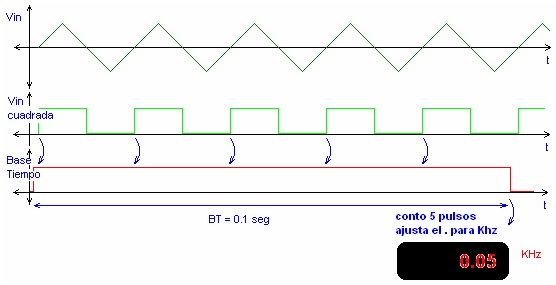
\includegraphics[width=0.70\textwidth]{images/ondasFrecuenciaContador.jpg}
	\medskip
\end{figure}
\bigskip\bigskip

	
	\medskip
	Diagrama de bloques para medir frecuencia:
	
	\begin{figure}[h]
				\centering
				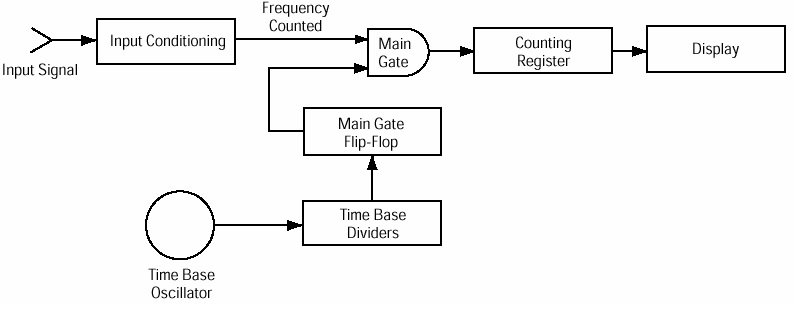
\includegraphics[width=0.47\textwidth]{images/diagramaBloquesFrecuenciaContador.jpg}
				\medskip
	\end{figure}
	\bigskip\bigskip
	
\subsection {Medicion de Período}
		
	\begin{figure}[h]
		\centering
		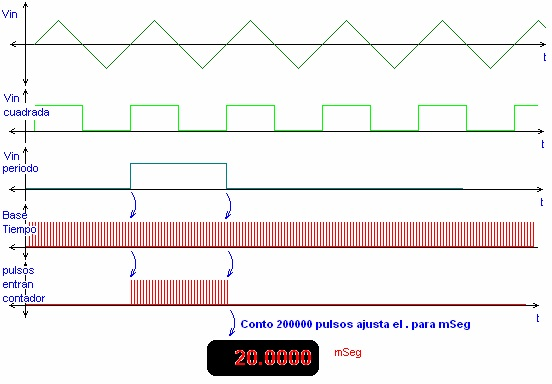
\includegraphics[width=0.47\textwidth]{images/ondasPeriodoContador.jpg}
		\medskip
	\end{figure}
	\bigskip\bigskip
	
	El contador cuenta la cantidad de pulsos de la base de tiempo durante un ciclo de la señal de entrada. A partir de ese valor obtiene el período.
	\medskip
	El diagrama en bloques del instrumento para poder realizar esta medición es:
		
		
	\begin{figure}[h]
		\centering
		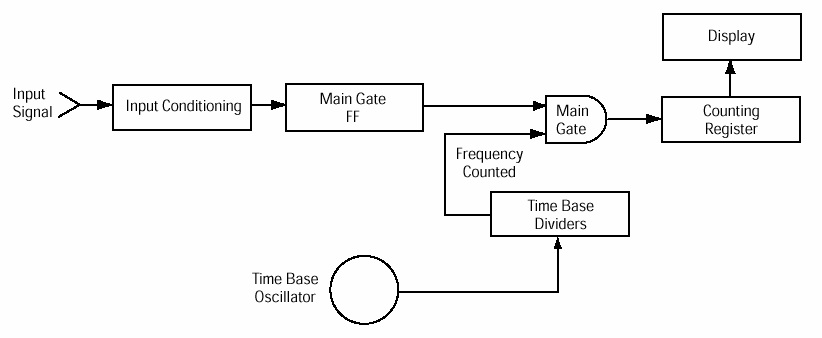
\includegraphics[width=0.47\textwidth]{images/diagramaBloquesPeriodoContador.jpg}
		\medskip
	\end{figure}
	\bigskip\bigskip
	
	
\subsection{Medición del Intervalo de tiempo}
	
	A diferencia de las mediciones anteriores, en este caso el objetivo de esta medición es medir el tiempo que transcurre entre dos eventos que pueden provenir de señales diferentes o de la misma señal.
	\medskip
	El diagrama en bloques del instrumento para poder realizar esta medición es:
	
	\begin{figure}[h]
		\centering
		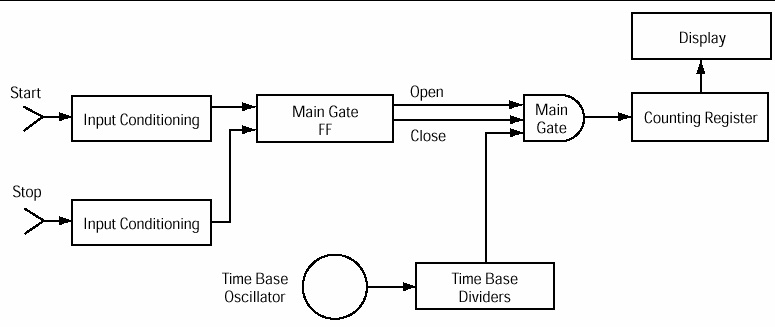
\includegraphics[width=0.47\textwidth]{images/diagramaBloquesIntervaloContador.jpg}
		\medskip
	\end{figure}
	\bigskip\bigskip
	
\subsection{Medición de la Relación de Frecuencias} 
	\medskip
	Esta última configuración permite comparar señales de frecuencias distintas, mostrando cuántos ciclos de una señal de alta frecuencia entran en un ciclo de la otra de frecuencia menor.
	\medskip
	El diagrama en bloques del instrumento para poder realizar esta medición es:
	
	\begin{figure}[h]
		\centering
		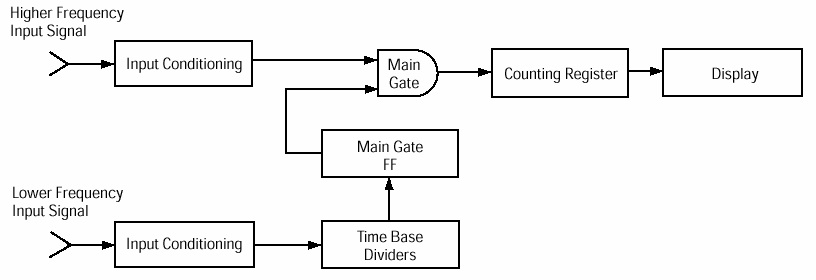
\includegraphics[width=0.47\textwidth]{images/diagramaBloquesRelacionContador.jpg}
		\medskip
	\end{figure}
	\bigskip\bigskip
	
	Incertezas en las mediciones
	\medskip
		Las mediciones realizadas están afectadas por incertezas debido al propio funcionamiento del instrumento y varían según el tipo de medición que se realiza.
		\medskip
		Los errores que pueden aparecer son:
			· Cuantización ó "±1 cuenta"
			· Disparo o trigger
			· Base de tiempo
			· Errores sistemáticos
	
\bigskip\bigskip




% MATERIALES UTILIZADOS
\section{Materiales utilizados}

	Se detalla a continuación (\textit{Tabla 1}) la lista de materiales y dispositivos utilizados durante el desarrollo de la práctica, acompañados por sus respectivas características y especificaciones principales. Para más información sobre el instrumental puede dirijirse a la sección \textit{Apéndice A}, ubicada al final del presente informe, donde se adjuntan las hojas de datos de todos estos.
\bigskip\bigskip


% Tabla 1
\begin{table}[!hbt]
	\begin{center}
	\begin{tabular}{|>{\centering\arraybackslash}m{5cm}|>{\arraybackslash}m{6cm}|}
		\hline
		\rowcolor[gray]{0.9}\textbf{Material/Instrumento} & \textbf{Especificaciones} \\
		\hline
		Generador de funciones & Modelo: 8140\\
		\hline
		Osciloscipio & \vbox{\hbox{\strut Marca: GOOD-WILL }
						   \hbox{\strut Modelo: 653G }}\\
		\hline
		Contador universal & \vbox{\hbox{\strut Marca: GOOD-WILL }
						   \hbox{\strut Modelo: GUC-2020 }}\\
		\hline
		Contador recíproco & \vbox{\hbox{\strut Marca: GOLDSTAR }
						   \hbox{\strut Modelo: FC-2130U / FC-2015U }}\\
		\hline
		Cables & Banana-Cocodrilo\newline Cocodrilo-Cocodrilo\newline BNC-BNC\newline Banana-BNC \\
		\hline
	\end{tabular}
	\caption{Listado de materiales e instrumental utilizado.}
	\end{center}
\end{table}
\bigskip\bigskip




% DESARROLLO
\section{Desarrollo}

	En los siguientes apartados se pasarán a desarrollar las mediciones empíricas, cada una de las cuales esta complementada con una explicación de los pasos llevados a cabo, valores obtenidos, análisis de resultados y conclusiones parciales.
\bigskip






%% DESARROLLO - Primer medición
\subsection{Primer medición}
	
	Banco de Medición:
	
	\begin{figure}[h]
				\centering
				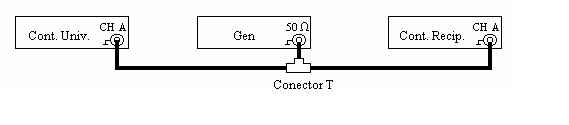
\includegraphics[width=0.47\textwidth]{images/bancoMedicion.jpg}
				\medskip
	\end{figure}
	\bigskip\bigskip	

	Para el desarrollo de esta medición se generó una onda cuadrada de amplitud 5V pico a pico, y se fue variando la frecuencia desde el generador de funciones y cambiando el modo y la base de tiempo de los contadores. Se obtuvo la siguiente tabla:

\newpage
% Tabla 2
\begin{table}[!hbt]
	\begin{center}

		\begin{tabular}{|c|c|c|c|c|c|c|} \hline
			\multirow{2}{*}{\textbf{Frecuencia}}
			& \multicolumn{2}{c|}{\textbf{Contador recíproco}} & \multicolumn{2}{c|}{\textbf{Contador universal}} & \multirow{2}{*}{\textbf{Modo}} & \multirow{2}{*}{\textbf{Gate Time}} \\\cline{2-5}
			& Indicación display & Error & Indicación display & Error & & \\\hline
			
			\multirow{4}{*}{\textbf{10 Hz}}
			& 9,991893 Hz &  & 0,010 KHz &  & Frecuencia & 1 Seg. \\\cline{2-7}
			& 100131,1 $\mu$S &  & ¿OVER? &  & Período & 1 Seg. \\\cline{2-7}
			& - &  & ¿GATE? &  & Frecuencia & 0.01 Seg. \\\cline{2-7}
			& - &  & 100201,7 $\mu$S &  & Período & 0.01 Seg. \\\hline

			\multirow{4}{*}{\textbf{1 kHz}}
			& 1,00423 kHz &  & 1,005 kHz &  & Frecuencia & 1 Seg. \\\cline{2-7}
			& 995,7958 $\mu$S &  & 995,797 $\mu$S &  & Período & 1 Seg. \\\cline{2-7}
			& 1,0036 kHz &  & 1,0 kHz &  & Frecuencia & 0.01 Seg. \\\cline{2-7}
			& 996,43 $\mu$S &  & 996,5 $\mu$S &  & Período & 0.01 Seg. \\\hline

			\multirow{4}{*}{\textbf{1 MHz}}
			& 1,001719 MHz &  & 1001,743 kHz &  & Frecuencia & 1 Seg. \\\cline{2-7}
			& 0,998182 $\mu$S &  & 0,998 $\mu$S &  & Período & 1 Seg. \\\cline{2-7}
			& 1,0015 MHz &  & 1001,5 kHz &  & Frecuencia & 0.01 Seg. \\\cline{2-7}
			& 0,99868 $\mu$S &  & 1,0 $\mu$S &  & Período & 0.01 Seg. \\\hline
		\end{tabular}

	\caption{Valores obtenidos en la primer medición.}
	\end{center}
\end{table}
\medskip




% Tabla 3
\begin{table}[!hbt]
	\begin{center}

		\begin{tabular}{|c|c|c|c|c|c|c|} \hline
			\multirow{2}{*}{\textbf{Frecuencia}}
			& \multicolumn{3}{c|}{\textbf{Contador universal}} & \multicolumn{3}{c|}{\textbf{Contador recíproco}} \\\cline{2-7}
			& Modo (\textit{f} ó \textit{T}) & Gate time & Error & Modo (\textit{f} ó \textit{T}) & Gate time & Error \\\hline
			
			\textbf{10 Hz} &  &  &  &  &  &  \\\hline
			\textbf{1 kHz} &  &  &  &  &  &  \\\hline
			\textbf{1 MHz} &  &  &  &  &  &  \\\hline
		\end{tabular}

	\caption{Valores calculados para la primer medición.}
	\end{center}
\end{table}
\medskip



%% DESARROLLO - Segunda medición
\subsection{Segunda medición}

	Banco de Medición:
	
	\begin{figure}[h]
				\centering
				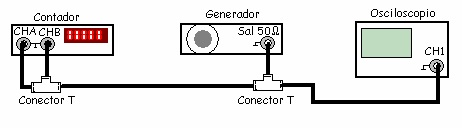
\includegraphics[width=0.47\textwidth]{images/bancoMedicionMed2.jpg}
				\medskip
	\end{figure}
	\bigskip\bigskip
	
	Para el desarrollo de esta medición se generó una onda cuadrada de amplitud 5V pico a pico, 1 KHz de frecuencia y se fue variando el ciclo de trabajo desde el generador y probando todas las combinaciones posibles entre el slope A y B ( + y -). 
\bigskip


% Tabla 4
\begin{table}[!hbt]
	\begin{center}

		\begin{tabular}{|c|c|c|c|c|c|c|c|c|c|c|} \hline
			\multirow{3}{*}{\textbf{Duty Cycle}}
			& \multicolumn{2}{c|}{\textbf{Slope A +}} & \multicolumn{2}{c|}{\textbf{Slope A +}} & \multicolumn{2}{c|}{\textbf{Slope A -}} & \multicolumn{2}{c|}{\textbf{Slope A -}} & \multicolumn{2}{c|}{\textbf{Duty Cycle}} \\
			& \multicolumn{2}{c|}{\textbf{Slope B +}} & \multicolumn{2}{c|}{\textbf{Slope B -}} & \multicolumn{2}{c|}{\textbf{Slope B +}} & \multicolumn{2}{c|}{\textbf{Slope B -}} & \multicolumn{2}{c|}{(calculado)} \\\cline{2-11}
			& \textbf{Display} & \textbf{Error} & \textbf{Display} & \textbf{Error} & \textbf{Display} & \textbf{Error} & \textbf{Display} & \textbf{Error} & \textbf{Valor} & \textbf{Error} \\\hline
			
			\textbf{20\%} & 996,34 &  & 263,78 &  & 730,77 &  & 994,57 &  &  &  \\\hline
			\textbf{50\%} & 998,35 &  & 509,70 &  & 502,35 &  & 13,84 &  &  &  \\\hline
			\textbf{80\%} & 1001,70 &  & 785,50 &  & 216,06 &  & 1002,65 &  &  &  \\\hline
		\end{tabular}

	\caption{Valores obtenidos en la segunda medición.}
	\end{center}
\end{table}
\medskip
	


%% DESARROLLO - Tercera medición
\subsection{Tercera medición}


% Tabla 5
\begin{table}[!hbt]
	\begin{center}
		\begin{tabular}{|c|c|c|} \hline
			\textbf{Frecuencia del generador} & \textbf{Lectura del display} & \textbf{Error} \\\hline
			100 Hz & 0,1 &  \\\hline
			1 kHz & 11 &  \\\hline
			10 kHz & 10,4 &  \\\hline
			100 kHz & 102,4 &  \\\hline
		\end{tabular}

	\caption{Valores obtenidos en la tercera medición.}
	\end{center}
\end{table}
\medskip


% Tabla 6
\begin{table}[!hbt]
	\begin{center}
		\begin{tabular}{|c|c|} \hline
			\multicolumn{2}{|c|}{\textbf{Frecuencia de la señal de calibración}} \\\cline{1-2}
			\textbf{Lectura del display} & \textbf{Error} \\\hline
			999,807 & \\\hline
		\end{tabular}

	\caption{Valores obtenidos en la tercera medición.}
	\end{center}
\end{table}
\medskip



%% DESARROLLO - Cuarta medición
\subsection{Cuarta medición}


% Tabla 7
\begin{table}[!hbt]
	\begin{center}

		\begin{tabular}{|c|c|c|c|c|c|c|} \hline
			\textbf{Frecuencia} & \multicolumn{2}{c|}{\textbf{Frecuencia medida}} & \multicolumn{2}{c|}{\textbf{Intervalo de tiempo medido}} & \multicolumn{2}{c|}{\textbf{desfasaje calculado}} \\\cline{2-7}
			\textbf{del generador} & Indicación display & Error & Indicación display & Error & Resultado & Error propagado \\\hline
			
			320 Hz & 326,6041 Hz & 0,31\% & 2978,705 $\mu$S & 0.0012\% & 16,93° & 0,31\% \\\hline
			1600 Hz & 1,611072 kHz & 0,06\% & 557,9888 $\mu$S & 0.0014\% & 36,01° & 0,06\% \\\hline
			8 kHz & 7,996636 kHz & 0,01\% & 96,55358 $\mu$S & 0.0022\% & 81,93° & 0,02\% \\\hline

		\end{tabular}

	\caption{Valores obtenidos en la cuarta medición.}
	\end{center}
\end{table}
\medskip



%% DESARROLLO - Quinta medición
\subsection{Quinta medición}


% Tabla 8
\begin{table}[!hbt]
	\begin{center}

		\begin{tabular}{|c|c|c|c|>{\centering}p{1.65cm}|c|} \hline
			\textbf{Amplitud} & \multicolumn{2}{c|}{\textbf{Tensión AC}} & \textbf{Lectura del} & \multicolumn{2}{c|}{\textbf{La medición es válida}} \\\cline{2-3}\cline{5-6}
			\textbf{sugerida} & \textbf{Lectura} & \textbf{Error} & \textbf{contador} & \textbf{Sí} & \textbf{No} \\\hline
			
			\textbf{5V} & 3,548 &  & 1,0 & \tick &  \\\hline
			\textbf{1V} & 0,677 &  & 1,1 &  &  \\\hline
			\textbf{0,5V} & 0,347 &  & 1,1 &  &  \\\hline
			\textbf{0,25V} & 0,173 &  & 1,2 &  &  \\\hline
			\textbf{0,05V} & 0,027 &  & 1,0 &  &  \\\hline
			\textbf{0,04V} & 0,019 &  & 0 &  &  \\\hline

		\end{tabular}

	\caption{Valores obtenidos en la quinta medición.}
	\end{center}
\end{table}
\medskip




% CONCLUSIONES
\section{Conclusiones}

% Tabla 9
\begin{table}[!hbt]
	\begin{center}
		\begin{tabular}{|c|c|c|c|} \hline
			\textbf{Equipo de medición} & \textbf{Frecuencia / Período} & \textbf{Desfasaje} & \textbf{Ancho de pulso} \\\hline
			Osciloscopio &  &  &  \\\hline
			Contador &  &  &  \\\hline
		\end{tabular}

	\caption{Cuadro comparativo de los ordenes de magnitud\\ de los errores de los equipos.}
	\end{center}
\end{table}
\medskip
	


\newpage \textit{}
\newpage



% APÉNDICE A
\newpage
\vspace*{4cm}
\begin{center}
	\textbf{\Huge{Apéndice A}} \\
	\bigskip\bigskip
	\Large{\textit{``Hojas de datos de instrumentos de medición''}}
\end{center}


\newpage \textit{}
\newpage

\end{document}
